\documentclass{standalone}
\usepackage{tikz}
\usetikzlibrary{arrows,positioning} 
\usetikzlibrary{fit}
\usetikzlibrary{shadows}




\tikzset{
	%Define standard arrow tip
	>=stealth',
	%Define style for boxes
	punkt/.style={
		rectangle,
		rounded corners,
		draw=black, very thick,
		text width=4.5em,
		minimum height=1.5em,
		text centered},
	% Define arrow style
	pil/.style={
		->,
		thick,
		shorten <=2pt,
		shorten >=2pt,}
}

\begin{document}
	
	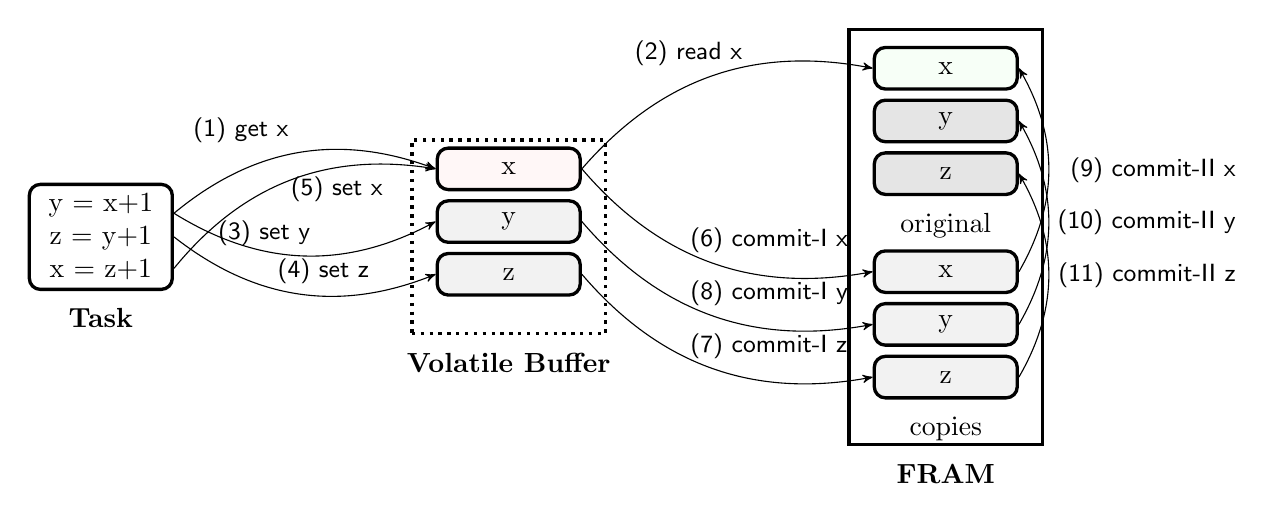
\begin{tikzpicture}[node distance=1cm, auto,]
	
	\node[punkt,minimum height=3em] (task1) {y = x+1 
		\\ z = y+1 \\ x = z+1};
	\node[below = 0.1cm of task1] () {\textbf{Task}};
		
	\node[draw,very thick,dotted,minimum width=7em, minimum height=7em, right = 3cm of task1] (sram) {};
	\node[below = 0.1cm of sram] () {\textbf{Volatile Buffer}};
	
	\node[punkt, below = -2.4cm of sram,fill=red!3] (x-sram) {x};
	\node[punkt, below = 0.1cm of x-sram,fill=black!5] (y-sram) {y};
	\node[punkt, below = 0.1cm of y-sram,fill=black!5] (z-sram) {z};

	\node[right = 1.8cm of sram] (ref) {};
	\node[draw,very thick,minimum width=7em, minimum height=15em, right = of ref] (fram1) {};
	
	
	%\node[draw,very thick,dotted,minimum width=7em, fill=green!5,minimum height=9em, below = 1cm of fram1] (fram2) {};
	
	
	\node[punkt, above = -0.8cm of fram1,fill=green!3] (x1-fram) {x};
	\node[punkt, below = 0.1cm of x1-fram,fill=black!10] (y1-fram) {y};
	\node[punkt, below = 0.1cm of y1-fram,fill=black!10] (z1-fram) {z};
	
	\node[punkt, below = -2.5cm of fram1,fill=black!5] (x2-fram) {x};
	\node[punkt, below = 0.1cm of x2-fram,fill=black!5] (y2-fram) {y};
	\node[punkt, below = 0.1cm of y2-fram,fill=black!5] (z2-fram) {z};

	\node[below = 0.1cm of z2-fram] (copies) {copies};	
	\node[below = 0.1cm of z1-fram] (original) {original};	
	\node[below = 0.7cm of z2-fram] () {\textbf{FRAM}};
	
	\path[every node/.style={font=\sffamily\small}]
	([yshift=0.3cm] task1.east) edge [->, bend left] node {(1) get x} (x-sram.west)
	(x-sram.east) edge [->, bend left] node[xshift=0.5cm] {(2) read x} (x1-fram.west)
	
	([yshift=0.3cm]task1.east) edge [->, bend right] node[xshift=-0.5cm] {(3) set y} (y-sram.west)
	
	(task1.east) edge [->, bend right] node[xshift=-0.4cm] {(4) set z} (z-sram.west)
	([yshift=-0.4cm]task1.east) edge [->, bend left] node[xshift=1.3cm,yshift=-0.4cm] {(5) set x} (x-sram.west)
	
	(x-sram.east) edge [->, bend right] node[xshift=-0.4cm] {(6) commit-I x} (x2-fram.west)
	(z-sram.east) edge [->, bend right] node[xshift=-0.4cm] {(7) commit-I z} (z2-fram.west)
	(y-sram.east) edge [->, bend right] node[xshift=-0.4cm] {(8) commit-I y} (y2-fram.west)
	
	(x2-fram.east) edge [->, bend right] node[xshift=2.5cm] {(9) commit-II x} (x1-fram.east)
	(y2-fram.east) edge [->, bend right] node[xshift=2.5cm] {(10) commit-II y} (y1-fram.east)
	(z2-fram.east) edge [->, bend right] node[xshift=2.5cm] {(11) commit-II z} (z1-fram.east)
	;
	
	\end{tikzpicture}
	
\end{document}